% -----------------------------*- LaTeX -*------------------------------
\documentclass[UTF8]{article}
% ------------------------------------------------------------------------
% Packages
% ------------------------------------------------------------------------
\usepackage{ctex} % 支持中文
\usepackage[body={7in, 9in},left=1in,right=1in]{geometry} % 改变页边距
\usepackage{amsmath} % AMS 的数学宏包
\usepackage{amsfonts} % AMS 的数学字体宏包
\usepackage{amssymb} % AMS 符号库
\usepackage{bm} % 数学公式中的黑斜体
\usepackage{amsthm} % AMS 的定理环境宏包
\usepackage{graphicx} % 插图
\usepackage{subfigure} % 插子图
\usepackage{nicefrac} % 好看的分数
\usepackage{mathrsfs} % mathscr font
\usepackage{caption} % caption
\usepackage{algorithm,algorithmicx} % 伪代码支持宏包
\usepackage[noend]{algpseudocode} % 伪代码
\usepackage{fancyhdr} % 设置页眉、页脚
\usepackage{adjustbox} % 图片尺寸自动调整
\usepackage{esint} % 积分符号
\usepackage{mathtools} % 数学宏包的重要补充
\usepackage{upgreek} % 数学环境的直立希腊字母
\usepackage{enumitem} % 使用enumitem宏包, 改变列表项的格式
\usepackage{color} % 支持彩色
\usepackage{extarrows} % 任意长度的箭头
\usepackage{tikz} % 绘图
\usepackage{forest} % 绘树
\usepackage{xcolor} % 颜色宏包
\usepackage{breqn} % 公式自动换行
\usepackage{fontsize} % 字体大小
\usepackage[framemethod=TikZ]{mdframed} % 给文字加框
\usepackage{fontspec} % 字体库
\usepackage{bigstrut} % 用于表格中的换行
\usepackage{multirow} % 表格中多行单元格合并
\usepackage{multicol} % 表格中多列单元格合并
\usepackage{longtable} % 长表格
\usepackage{rotating} % 旋转图形和表格      以上三者用于绘制三线表
\usepackage{booktabs} % 三线表宏包
\usepackage{scribe} % Scribe 模板
\usepackage{diagbox} % 表格斜线
\usepackage{listings} % 插入代码
\usetikzlibrary{automata} % 引入automata库
\usetikzlibrary{shapes,arrows,positioning,chains} % 引入positioning库
% ------------------------------------------------------------------------
% Macros
% ------------------------------------------------------------------------
%~~~~~~~~~~~~~~~
% Utility latin
%~~~~~~~~~~~~~~~
\newcommand{\ie}{\textit{i.e.}}
\newcommand{\eg}{\textit{e.g.}}
%~~~~~~~~~~~~~~~
% Environment shortcuts
%~~~~~~~~~~~~~~~
\newcommand{\balign}[1]{\ealign{\begin{align}#1\end{align}}}
\newcommand{\baligns}[1]{\ealigns{\begin{align*}#1\end{align*}}}
\newcommand{\bitemize}[1]{\eitemize{\begin{itemize}#1\end{itemize}}}
\newcommand{\benumerate}[1]{\eenumerate{\begin{enumerate}#1\end{enumerate}}}
%~~~~~~~~~~~~~~~
% Text with quads around it
%~~~~~~~~~~~~~~~
\newcommand{\qtext}[1]{\quad\text{#1}\quad}
%~~~~~~~~~~~~~~~
% Shorthand for math formatting
%~~~~~~~~~~~~~~~
\newcommand{\mbb}[1]{\mathbb{#1}}
\newcommand{\mbi}[1]{\boldsymbol{#1}} % Bold and italic (math bold italic)
\newcommand{\mbf}[1]{\mathbf{#1}}
\newcommand{\mc}[1]{\mathcal{#1}}
\newcommand{\mrm}[1]{\mathrm{#1}}
\newcommand{\tbf}[1]{\textbf{#1}}
\newcommand{\tsc}[1]{\textsc{#1}}
%\def\\langle {{\langle }}
%\def\\rangle {{\rangle }}
\newcommand{\sT}{\sf T}
\newcommand{\grad}{\nabla}
\newcommand{\Proj}{\Pi}
%~~~~~~~~~~~~~~~
% Common sets 定义数集符号
%~~~~~~~~~~~~~~~
\newcommand{\R}{\mathbb{R}}
\newcommand{\Z}{\mathbb{Z}}
\newcommand{\Q}{\mathbb{Q}}
\newcommand{\N}{\mathbb{N}}
\newcommand{\C}{\mathbb{C}}
\newcommand{\reals}{\mathbb{R}} % Real number symbol
\newcommand{\integers}{\mathbb{Z}} % Integer symbol
\newcommand{\rationals}{\mathbb{Q}} % Rational numbers
\newcommand{\naturals}{\mathbb{N}} % Natural numbers
\newcommand{\complex}{\mathbb{C}} % Complex numbers
%~~~~~~~~~~~~~~~
% Common functions
%~~~~~~~~~~~~~~~
\renewcommand{\exp}[1]{\operatorname{exp}\left(#1\right)} % Exponential
\newcommand{\indic}[1]{\mbb{I}\left(#1\right)} % Indicator function
\newcommand{\indicsub}[2]{\mbb{I}_{#2}\left(#1\right)} % Indicator function
\newcommand{\argmax}{\mathop\mathrm{arg\, max}} % Defining math symbols
\newcommand{\argmin}{\mathop\mathrm{arg\, min}}
\renewcommand{\arccos}{\mathop\mathrm{arccos}}
\newcommand{\dom}{\mathop\mathrm{dom}} % Domain
\newcommand{\range}{\mathop\mathrm{range}} % Range
\newcommand{\diag}{\mathop\mathrm{diag}}
\newcommand{\tr}{\mathop\mathrm{tr}}
\newcommand{\abs}{\mathop\mathrm{abs}}
\newcommand{\card}{\mathop\mathrm{card}}
\newcommand{\sign}{\mathop\mathrm{sign}}
\newcommand{\prox}{\mathrm{prox}} % prox
\newcommand{\rank}[1]{\mathrm{rank}(#1)}
\newcommand{\supp}[1]{\mathrm{supp}(#1)}
\newcommand{\norm}[1]{\lVert#1\rVert}
%~~~~~~~~~~~~~~~
% Common probability symbols
%~~~~~~~~~~~~~~~
\newcommand{\family}{\mathcal{P}} % probability family / statistical model
\newcommand{\iid}{\stackrel{\mathrm{iid}}{\sim}}
\newcommand{\ind}{\stackrel{\mathrm{ind}}{\sim}}
\newcommand{\E}{\mathbb{E}} % Expectation symbol
\newcommand{\Earg}[1]{\E\left[#1\right]}
\newcommand{\Esubarg}[2]{\E_{#1}\left[#2\right]}
\renewcommand{\P}{\mathbb{P}} % Probability symbol
\newcommand{\Parg}[1]{\P\left(#1\right)}
\newcommand{\Psubarg}[2]{\P_{#1}\left[#2\right]}
%\newcommand{\Cov}{\mrm{Cov}} % Covariance symbol
%\newcommand{\Covarg}[1]{\Cov\left[#1\right]}
%\newcommand{\Covsubarg}[2]{\Cov_{#1}\left[#2\right]}
%\newcommand{\model}{\mathcal{P}} % probability family / statistical model
%~~~~~~~~~~~~~~~
% Distributions
%~~~~~~~~~~~~~~~
%\newcommand{\Gsn}{\mathcal{N}}
%\newcommand{\Ber}{\textnormal{Ber}}
%\newcommand{\Bin}{\textnormal{Bin}}
%\newcommand{\Unif}{\textnormal{Unif}}
%\newcommand{\Mult}{\textnormal{Mult}}
%\newcommand{\NegMult}{\textnormal{NegMult}}
%\newcommand{\Dir}{\textnormal{Dir}}
%\newcommand{\Bet}{\textnormal{Beta}}
%\newcommand{\Gam}{\textnormal{Gamma}}
%\newcommand{\Poi}{\textnormal{Poi}}
%\newcommand{\HypGeo}{\textnormal{HypGeo}}
%\newcommand{\GEM}{\textnormal{GEM}}
%\newcommand{\BP}{\textnormal{BP}}
%\newcommand{\DP}{\textnormal{DP}}
%\newcommand{\BeP}{\textnormal{BeP}}
%\newcommand{\Exp}{\textnormal{Exp}}
%~~~~~~~~~~~~~~~
% Theorem-like environments
%~~~~~~~~~~~~~~~
%\theoremstyle{definition}
%\newtheorem{definition}{Definition}
%\newtheorem{example}{Example}
%\newtheorem{problem}{Problem}
%\newtheorem{lemma}{Lemma}
%~~~~~~~~~~~~~~~
% 组合数学的模板和作业里用到的一些宏包和自定义命令
%~~~~~~~~~~~~~~~
\renewcommand{\emph}[1]{\begin{kaishu}#1\end{kaishu}}
\newcommand{\falfac}[1]{^{\underline{#1}}}
\newcommand{\binomfrac}[2]{\frac{#1^{\underline{#2}}}{#2!}}
\newcommand{\ceil}[1]{\left\lceil #1 \right\rceil}
\newcommand{\floor}[1]{\left\lfloor #1 \right\rfloor}
\newcommand{\suminfty}[2]{\sum_{#1=#2}^{\infty}}
\newcommand{\suminftyk}[0]{\sum_{k=0}^{\infty}}
\newcommand{\sumint}[3]{\sum_{#1=#2}^{#3}}
\newcommand{\sumintk}[2]{\sum_{k=#1}^{#2}}
\newcommand{\suminti}[2]{\sum_{i=#1}^{#2}}
%~~~~~~~~~~~~~~~
% 定义新命令
%~~~~~~~~~~~~~~~
\newcommand*{\unit}[1]{\mathop{}\!\mathrm{#1}}
\newcommand*{\dif}{\mathop{}\!\mathrm{d}}%微分算子 d
\newcommand*{\pdif}{\mathop{}\!\partial}%偏微分算子
\newcommand*{\cdif}{\mathop{}\!\nabla}%协变导数、nabla 算子
\newcommand*{\laplace}{\mathop{}\!\Delta}%laplace 算子
\newcommand*{\deri}[1]{\mathrm{d} #1}
\newcommand*{\deriv}[2]{\frac{\mathrm{d} #1}{\mathrm{d} {#2}}}
\newcommand*{\derivh}[3]{\frac{\mathrm{d}^{#1} #2}{\mathrm{d} {#3^{#1}}}}
\newcommand*{\pderiv}[2]{\frac{\partial #1}{\partial {#2}}}
\newcommand*{\pderivh}[3]{\frac{\partial^{#1} #2}{\partial {#3^{#1}}}}
\newcommand*{\dderiv}[2]{\dfrac{\mathrm{d} #1}{\mathrm{d} {#2}}}
\newcommand*{\dderivh}[3]{\dfrac{\mathrm{d}^{#1} #2}{\mathrm{d} {#3^{#1}}}}
\newcommand*{\dpderiv}[2]{\dfrac{\partial #1}{\partial {#2}}}
\newcommand*{\dpderivh}[3]{\dfrac{\partial^{#1} #2}{\partial {#3^{#1}}}}
\newcommand{\me}[1]{\mathrm{e}^{#1}}%e 指数
\newcommand{\mi}{\mathrm{i}}%虚数单位
%\newcommand{\mc}{\mathrm{c}}%光速 定义与mathcal冲突
\newcommand{\red}[1]{\textcolor{red}{#1}}
\newcommand{\blue}[1]{\textcolor{blue}{#1}}
%\newcommand{\Rome}[1]{\setcounter{rome}{#1}\Roman{rome}}
%~~~~~~~~~~~~~~~
% 公式环境中箭头符号的简写
%~~~~~~~~~~~~~~~
\newcommand{\ra}{\rightarrow}
\newcommand{\Ra}{\Rightarrow}
\newcommand{\la}{\leftarrow}
\newcommand{\La}{\Leftarrow}
\newcommand{\lra}{\leftrightarrow}
\newcommand{\Lra}{\Leftrightarrow}
\newcommand{\lgla}{\longleftarrow}
\newcommand{\Lgla}{\Longleftarrow}
\newcommand{\lgra}{\longrightarrow}
\newcommand{\Lgra}{\Longrightarrow}
\newcommand{\lglra}{\longleftrightarrow}
\newcommand{\Lglra}{\Longleftrightarrow}
%~~~~~~~~~~~~~~~
% 一些数学的环境设置
%~~~~~~~~~~~~~~~
%\newcounter{counter_exm}\setcounter{counter_exm}{1}
%\newcounter{counter_prb}\setcounter{counter_prb}{1}
%\newcounter{counter_thm}\setcounter{counter_thm}{1}
%\newcounter{counter_lma}\setcounter{counter_lma}{1}
%\newcounter{counter_dft}\setcounter{counter_dft}{1}
%\newcounter{counter_clm}\setcounter{counter_clm}{1}
%\newcounter{counter_cly}\setcounter{counter_cly}{1}
\newtheorem{theorem}{{\hskip 1.7em \bf 定理}}
\newtheorem{lemma}[theorem]{\hskip 1.7em 引理}
\newtheorem{proposition}[theorem]{\hskip 1.7em 命题}
\newtheorem{claim}[theorem]{\hskip 1.7em 断言}
\newtheorem{corollary}[theorem]{\hskip 1.7em 推论}
% \newcommand{\problem}[1]{{\setlength{\parskip}{10pt}\noindent \bf{#1}}}
\newenvironment{solution}{{\noindent \bf 解 \quad}}{}
\newenvironment{remark}{{\noindent \bf 注 \quad}}{}
\newenvironment{definition}{{\noindent \bf 定义 \quad}}{}
\renewenvironment{proof}{{\setlength{\parskip}{7pt}\noindent\hskip 2em \bf 证明 \quad}}{\hfill$\qed$\par}
\newenvironment{example}{{\noindent\bf 例 \quad}}{\hfill$\qed$\par}
%\newenvironment{concept}[1]{{\bf #1\quad} \begin{kaishu}} {\end{kaishu}\par}
%~~~~~~~~~~~~~~~
% 本.tex文档中特殊定义命令
%~~~~~~~~~~~~~~~
\newcommand{\lno}[1]{\overline{#1}}
\newcommand{\NP}{\mathrm{NP}}
\newcommand{\coNP}{\mathrm{coNP}}
% \newcommand{\ISO}{\mathrm{ISO}}
\newcommand{\SAT}{\mathrm{SAT}}
\newcommand{\USAT}{\mathrm{USAT}}
% \newcommand{\threeSAT}{\mathrm{3\text{-}SAT}}
\renewcommand{\P}{\mathrm{P}}
% \mathchardef\mhyphen="2D
% \newcommand{\CNF}{\mathrm{CNF}}
% \newcommand{\DNF}{\mathrm{DNF}}
% \newcommand{\SetSp}{\mathrm{SET\text{-}SPLITTING}}
% \newcommand{\PUZZLE}{\mathrm{PUZZLE}}
% \newcommand{\SPATH}{\mathrm{SPATH}}
% \newcommand{\LPATH}{\mathrm{LPATH}}
% \newcommand{\UHAMPATH}{\mathrm{UHAMPATH}}
\newcommand{\SPACE}{\mathrm{SPACE}}
\newcommand{\NSPACE}{\mathrm{NSPACE}}
\newcommand{\PSPACE}{\mathrm{PSPACE}}
\newcommand{\NPSPACE}{\mathrm{NPSPACE}}
\newcommand{\DFA}{\mathrm{DFA}}
\newcommand{\NFA}{\mathrm{NFA}}
\newcommand{\TQBF}{\mathrm{TQBF}}
% \newcommand{\L}{\mathrm{L}}
\renewcommand{\O}{\mathrm{O}}
\newcommand{\NL}{\mathrm{NL}}
\newcommand{\coNL}{\mathrm{coNL}}
\newcommand{\LADDER}{\mathrm{LADDER_{DFA}}}
\newcommand{\hd}{\mathrm{\text{-}hard}}
\newcommand{\ADD}{\mathrm{ADD}}
\newcommand{\STCN}{\mathrm{STRONGLY\text{-}CONNECTED}}
\newcommand{\PATH}{\mathrm{PATH}}
\newcommand{\A}{\mathrm{A}}
%使用align环境公式换页
\allowdisplaybreaks[4]

\definecolor{dkgreen}{rgb}{0,0.6,0}
\definecolor{gray}{rgb}{0.5,0.5,0.5}
\definecolor{mauve}{rgb}{0.58,0,0.82}
\lstset{
  frame=tb,
  aboveskip=3mm,
  belowskip=3mm,
  showstringspaces=false,
  columns=flexible,
  framerule=1pt,
  rulecolor=\color{gray!35},
  backgroundcolor=\color{gray!5},
  basicstyle={\small\ttfamily},
  numbers=none,
  numberstyle=\tiny\color{gray},
  keywordstyle=\color{blue},
  commentstyle=\color{dkgreen},
  stringstyle=\color{mauve},
  breaklines=true,
  breakatwhitespace=true,
  tabsize=3,
}

\setmainfont{Times New Roman}
\setsansfont{Times New Roman}
\setmonofont{Consolas}
\setCJKmainfont{SimHei}
\setCJKsansfont{SimSun}
\setCJKmonofont{FangSong}
\punctstyle{kaiming}

\begin{document}

\pagestyle{fancy}
\lhead{\emph{计算机网络实验课}}
\chead{\emph{中国科学院大学}}
\rhead{\emph{2022K800992910张家玮}}

\begin{center}
    {\LARGE \bf 第一次实验}
\end{center}

\section{互联网协议实验}

\subsection{实验内容}

使用wireshark抓包工具,用wget下载www.ucas.ac.con,观察输出。根据输出分析ARP、DNS、TCP、HTTP协议的工作过程。

\subsection{实验步骤}

在ubuntu虚拟机终端中依次输入以下命令:

\begin{lstlisting}[language=bash]
  sudo mn --nat # 启动mininet
  xterm h1 # 打开h1终端
  echo "nameserver 1.2.4.8" > /etc/resolv.conf # 设置DNS服务器
  wireshark & # 打开wireshark,然后选择h1-eth0开始抓包
  wget www.ucas.ac.cn # h1中输入该指令,下载网页,开始调研
\end{lstlisting}

\subsection{实验结果}

如下图所示:

\begin{figure}[H]
  \centering
  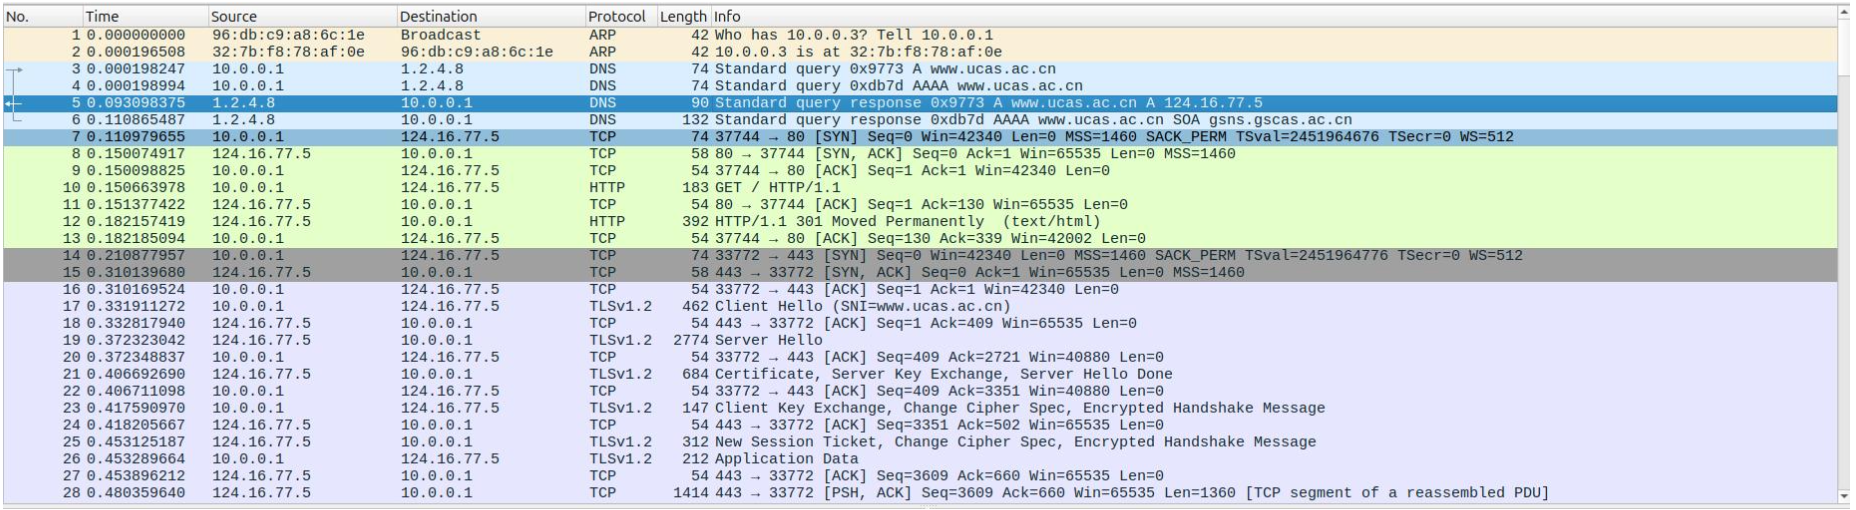
\includegraphics[width=\textwidth]{result1.png}
  \caption{wireshark抓包结果}
\end{figure}

然后进入各个协议中查看详细信息,如下几张图所示:

\begin{figure}[H]
  \centering
  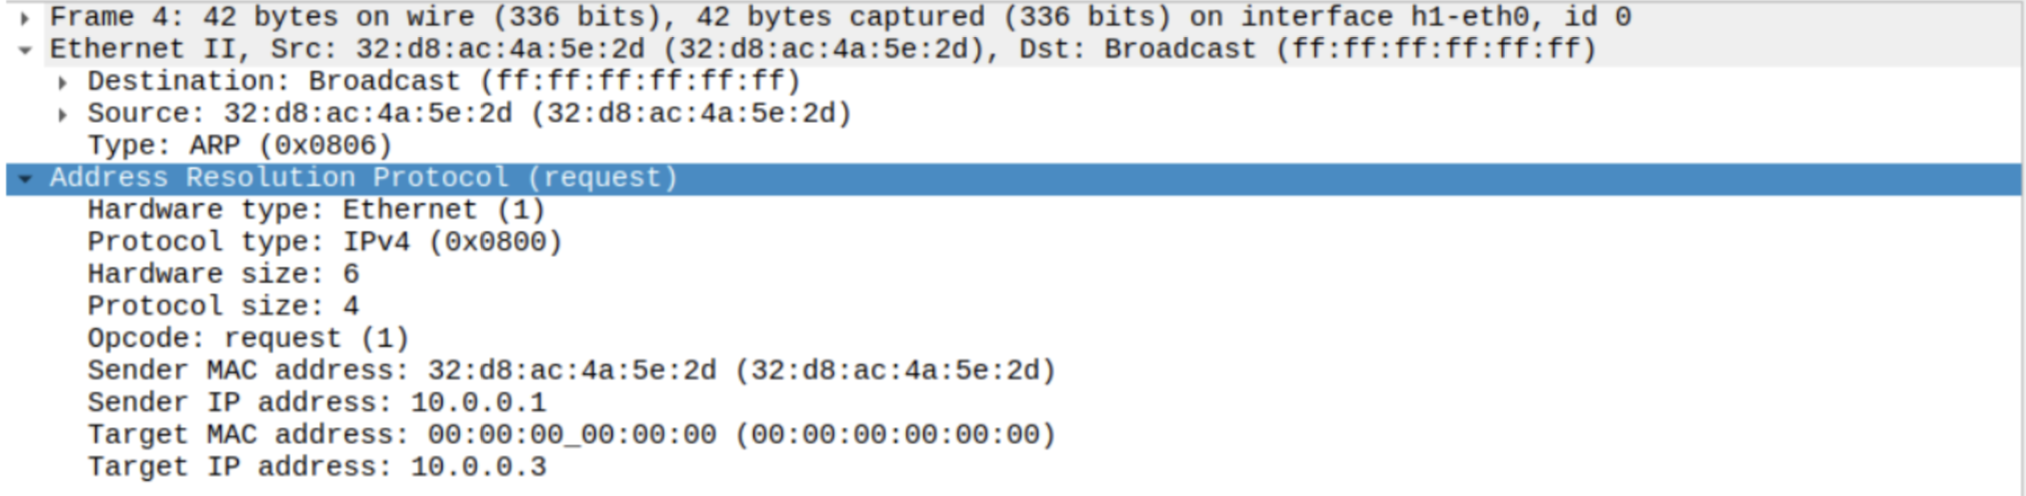
\includegraphics[width=\textwidth]{ARP.png}
  \caption{ARP协议}
\end{figure}

\begin{figure}[H]
  \centering
  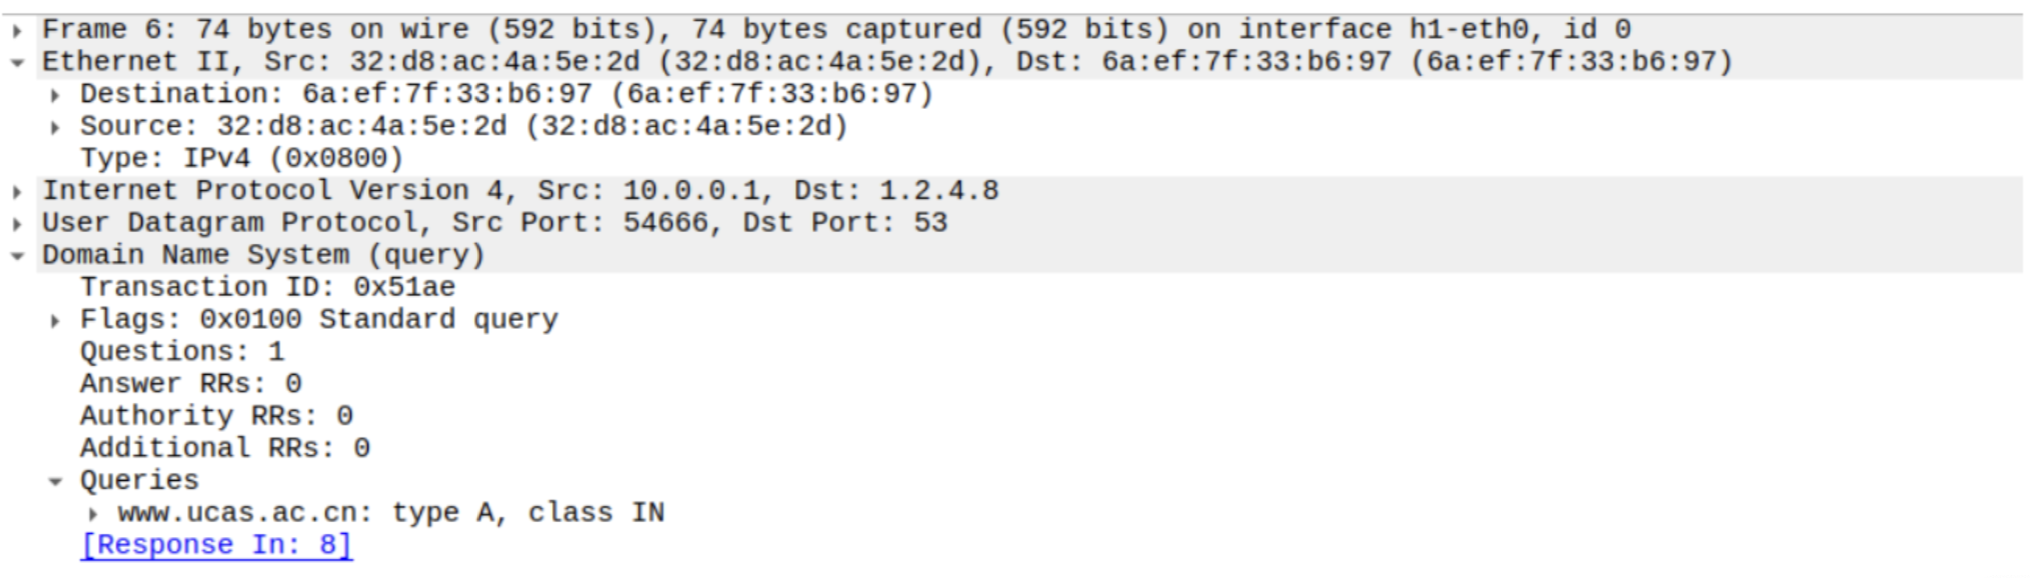
\includegraphics[width=\textwidth]{DNS.png}
  \caption{DNS协议}
\end{figure}

\begin{figure}[H]
  \centering
  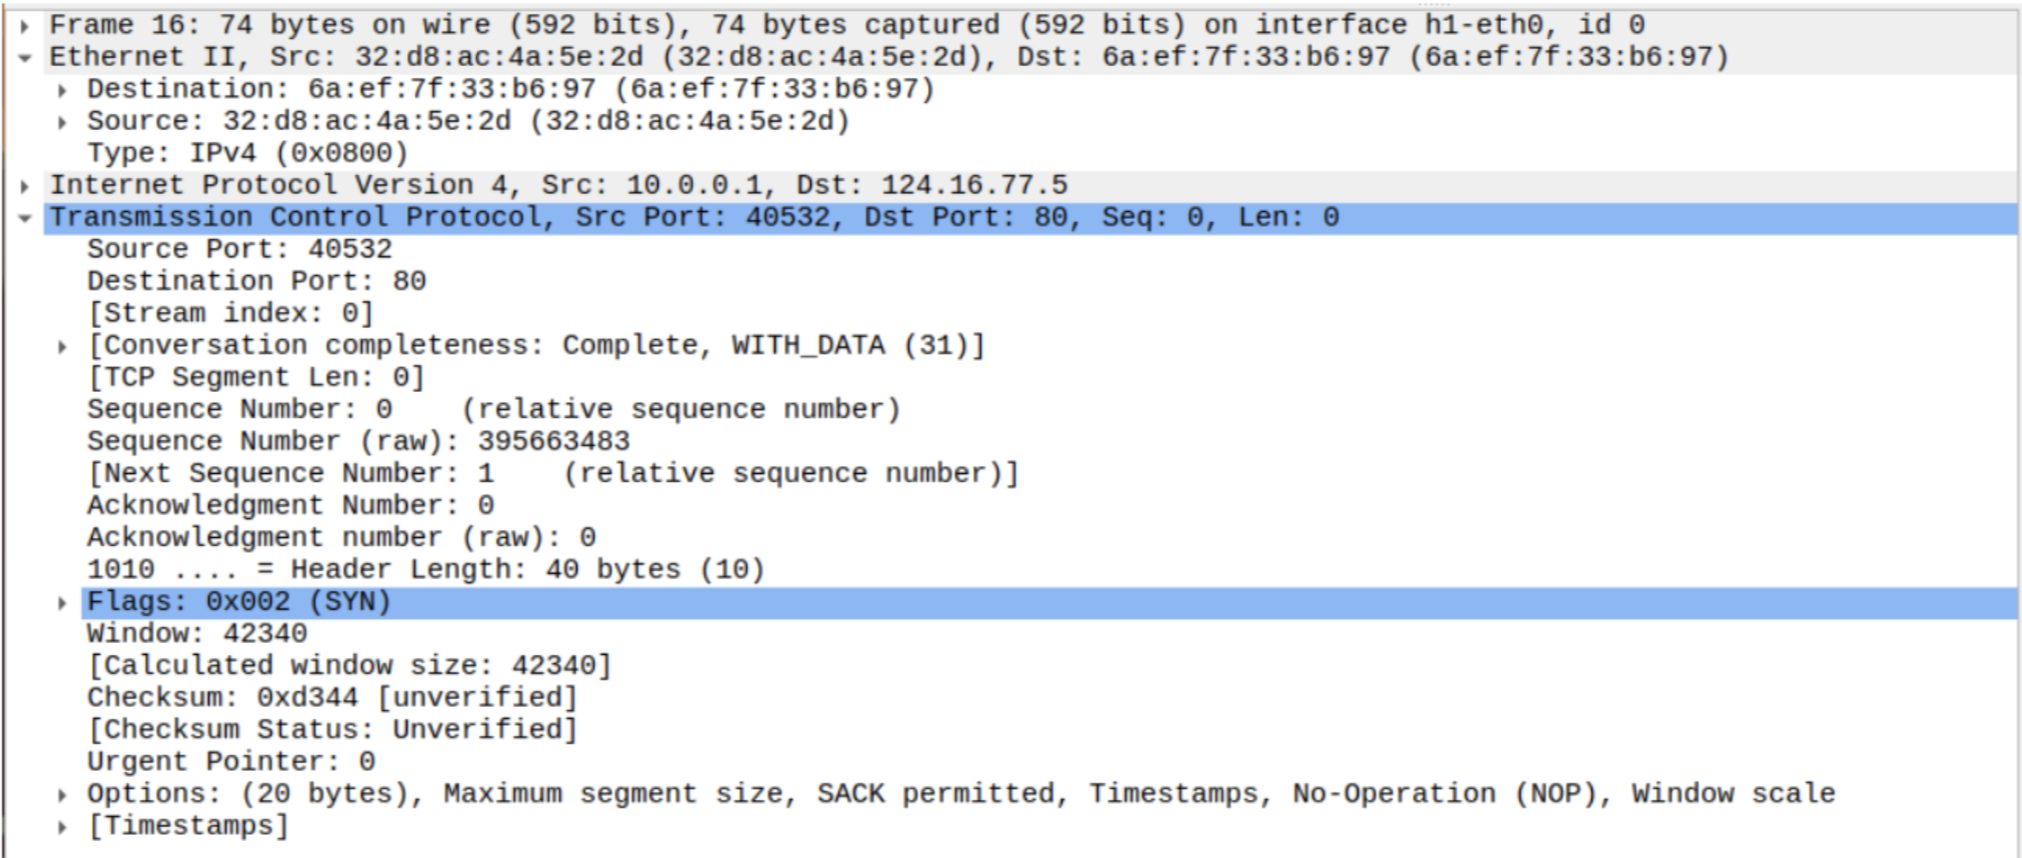
\includegraphics[width=\textwidth]{TCP.png}
  \caption{TCP协议}
\end{figure}

\begin{figure}[H]
  \centering
  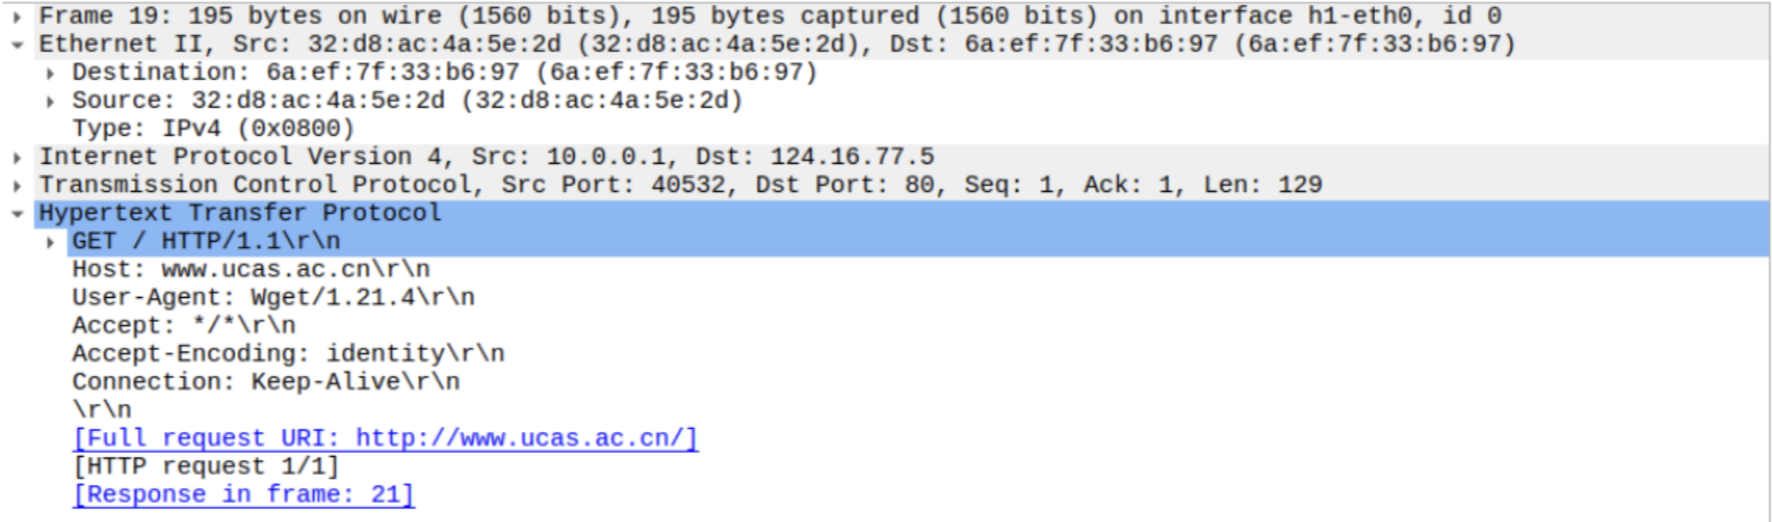
\includegraphics[width=\textwidth]{HTTP.png}
  \caption{HTTP协议}
\end{figure}

还得到了TCP流的详细信息:

\begin{figure}[H]
  \centering
  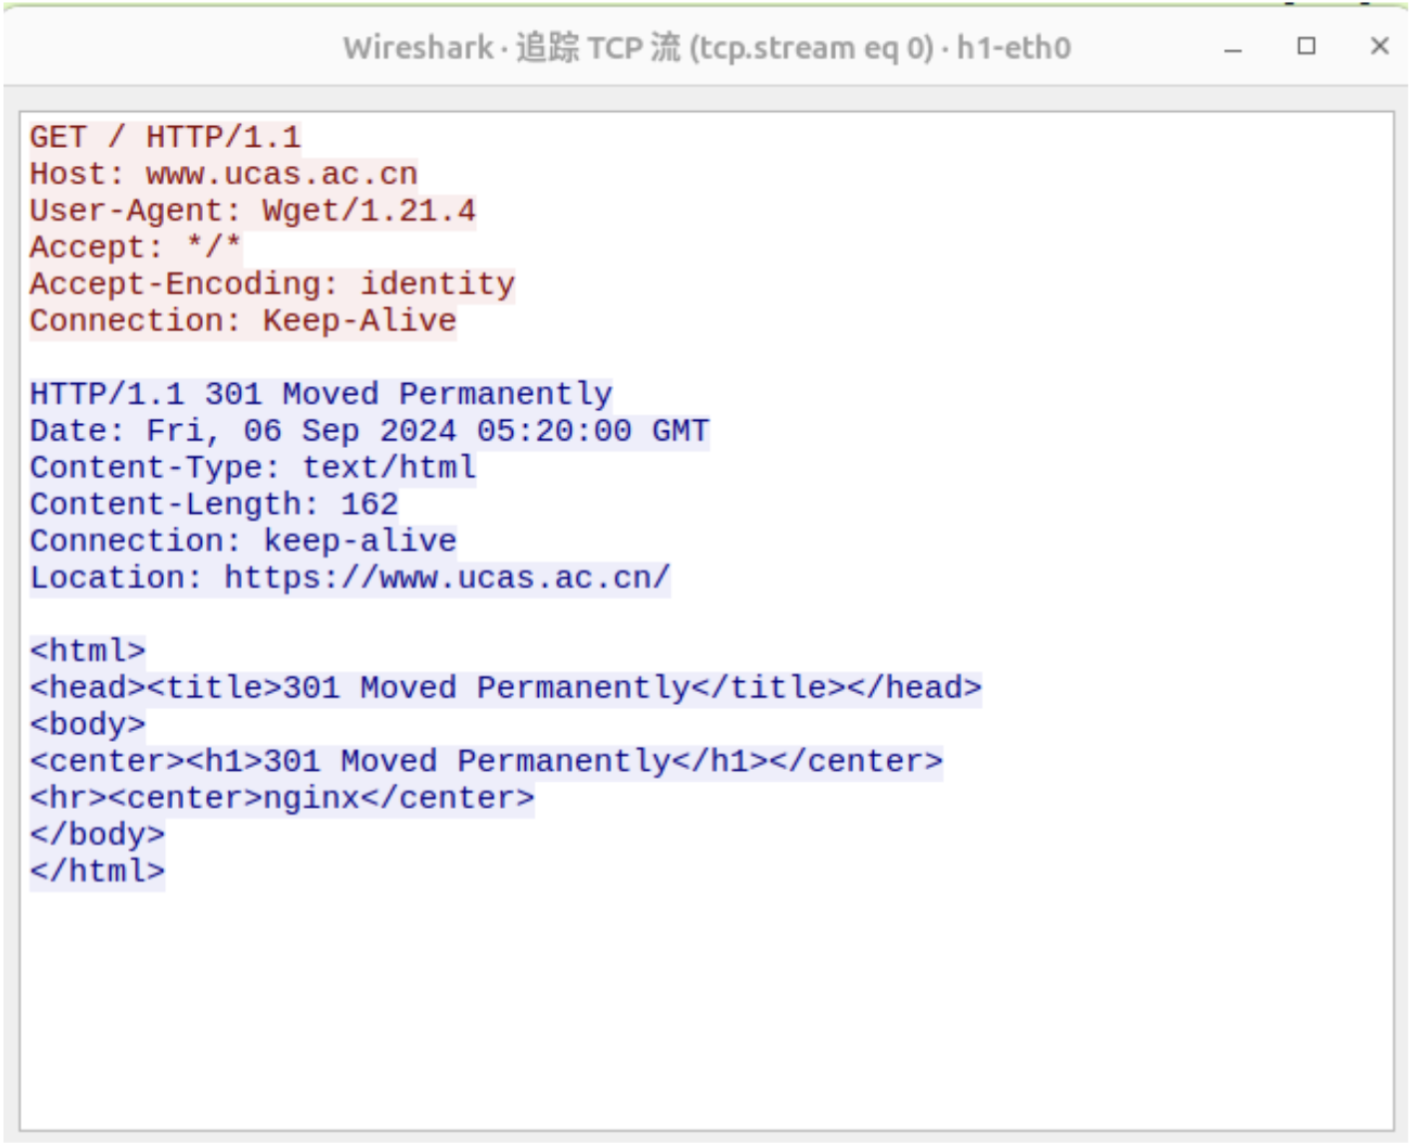
\includegraphics[width=\textwidth]{TCPflow.png}
  \caption{TCP流}
\end{figure}

\subsection{实验分析}

在抓包过程中,我们可以看到获取目标网页的过程中,总共使用了四种协议,即ARP、DNS、TCP和HTTP协议。封装层次总结如下:

\begin{enumerate}
  \item ARP协议:Ethernet < ARP;
  \item DNS协议:Ethernet < IPv4 < UDP < DNS;
  \item TCP协议:Ethernet < IPv4 < TCP;
  \item HTTP协议:Ethernet < IPv4 < TCP < HTTP;
\end{enumerate}

\subsection{实验解释}

ARP(地址解析协议,Address Resolution Protocol)是一种用于将网络层地址(如 IP 地址)解析为链路层地址(如 MAC 地址)的协议。它在局域网(LAN)中非常重要,尤其是在以太网中。当一台主机需要发送数据到另一台主机时,它首先需要知道目标主机的 MAC 地址。如果它不知道目标主机的 MAC 地址,它会广播一个 ARP 请求包到网络中,网络中拥有该 IP 地址的主机会回复一个 ARP 响应包,告知其 MAC 地址,随后主机会将 IP 地址和对应的 MAC 地址缓存起来,以便下次通信时不需要再次发送 ARP 请求。

DNS(域名系统,Domain Name System)协议用于将人类可读的域名解析为机器可读的 IP 地址。它是互联网的重要组成部分,允许用户通过域名访问网站,而不需要记住复杂的 IP 地址。当用户在浏览器中输入一个域名时,浏览器会首先检查本地缓存中是否有该域名的 IP 地址。如果没有,它会向本地 DNS 服务器发送一个 DNS 查询请求。本地 DNS 服务器会检查自己的缓存,如果没有找到对应的 IP 地址,它会向根 DNS 服务器发送查询请求。根 DNS 服务器会返回一个顶级域(如 .com)的 DNS 服务器地址。如果还是找不到,本地 DNS 服务器会继续向顶级域 DNS 服务器发送查询请求,直到找到负责该域名的权威 DNS 服务器,并获取最终的 IP 地址,本地 DNS 服务器将 IP 地址返回给用户的浏览器,浏览器使用该 IP 地址与目标服务器建立连接。

TCP(传输控制协议,Transmission Control Protocol)是一种面向连接的、可靠的传输层协议。它提供了可靠的数据传输服务,确保数据包按顺序到达,并且没有丢失或重复。TCP 使用三次握手来建立连接:客户端发送一个 SYN(同步)包到服务器;服务器收到 SYN 包后,回复一个 SYN-ACK(同步-确认)包;客户端收到 SYN-ACK 包后,回复一个 ACK(确认)包,连接建立完成。在连接建立后,TCP 使用序列号和确认号来确保数据包按顺序到达,并且没有丢失或重复。每个数据包都有一个序列号,接收方会发送一个确认号来确认已收到的数据。TCP 使用四次挥手来终止连接:一方发送一个 FIN(终止)包,表示不再发送数据;另一方收到 FIN 包后,回复一个 ACK 包;另一方也发送一个 FIN 包,表示不再发送数据;最后一方收到 FIN 包后,回复一个 ACK 包,连接终止完成。


HTTP(超文本传输协议,HyperText Transfer Protocol)是一种用于在客户端和服务器之间传输超文本的应用层协议。它是万维网(WWW)的基础,定义了客户端(通常是浏览器)如何向服务器请求资源以及服务器如何响应这些请求。HTTP 是无状态协议,每个请求都是独立的,与之前的请求没有关联。服务器不会保留任何关于客户端的状态信息。HTTP 使用请求-响应模型。客户端发送一个 HTTP 请求,服务器处理请求并返回一个 HTTP 响应。请求和响应都包含头部信息和可选的主体内容。HTTP 响应包含一个状态码,用于表示请求的结果。

\section{流完成时间实验}

\subsection{实验内容}

在给定带宽、延迟和文件大小前提下,查看流完成时间,变化文件大小(10MB, 100MB)、带宽(10Mbps, 100Mbps, 1Gbps)、延迟(100ms),查看不同条件下的流完成时间。利用fct_exp.py脚本,重现PPT中的实验结果。

\subsection{实验步骤}

在fct_exp.py文件中设置好带宽和延迟参数值之后,依次输入以下命令:

\begin{lstlisting}[language=bash]
  sudo python3 fct_exp.py # 运行fct_exp.py脚本
  xterm h1 h2 # 启动两个host
  dd if=/dev/zero of=1MB.dat bs=1M count=1 # 在h2中生成1MB的文件
  wget http://10.0.0.2/1MB.dat # 在h1中下载1MB的文件,记录时间和速度(文件大小更换为10MB和100MB)
\end{lstlisting}

\subsection{实验结果}

\begin{table}[H]
  \centering
  \caption{带宽为10Mbps、文件大小为1MB时的流完成时间}
  \begin{tabular}{|c|c|c|}
    \hline
    \multirow{3}{*}{序号}&带宽/Mbps&文件大小/MB\\
    \cline{2-3}
    &10&1\\
    \cline{2-3}
    &速率/Mbps&时间/s\\
    \hline
    1&4.88&1.7\\
    \hline
    2&5.04&1.6\\
    \hline
    3&4.984&1.6\\
    \hline
    均值&4.968&1.633333333\\
    \hline
  \end{tabular}
\end{table}

\begin{table}[H]
  \centering
  \caption{带宽为50Mbps、文件大小为1MB时的流完成时间}
  \begin{tabular}{|c|c|c|}
    \hline
    \multirow{3}{*}{序号}&带宽/Mbps&文件大小/MB\\
    \cline{2-3}
    &50&1\\
    \cline{2-3}
    &速率/Mbps&时间/s\\
    \hline
    1&6.224&1.3\\
    \hline
    2&6.608&1.2\\
    \hline
    3&5.592&1.5\\
    \hline
    均值&6.141333333&1.333333333\\
    \hline
  \end{tabular}
\end{table}

\begin{table}[H]
  \centering
  \caption{带宽为100Mbps、文件大小为1MB时的流完成时间}
  \begin{tabular}{|c|c|c|}
    \hline
    \multirow{3}{*}{序号}&带宽/Mbps&文件大小/MB\\
    \cline{2-3}
    &100&1\\
    \cline{2-3}
    &速率/Mbps&时间/s\\
    \hline
    1&6.456&1.3\\
    \hline
    2&5.648&1.5\\
    \hline
    3&4.944&1.7\\
    \hline
    均值&5.682666667&1.5\\
    \hline
  \end{tabular}
\end{table}

\begin{table}[H]
  \centering
  \caption{带宽为500Mbps、文件大小为1MB时的流完成时间}
  \begin{tabular}{|c|c|c|}
    \hline
    \multirow{3}{*}{序号}&带宽/Mbps&文件大小/MB\\
    \cline{2-3}
    &500&1\\
    \cline{2-3}
    &速率/Mbps&时间/s\\
    \hline
    1&5.768&1.4\\
    \hline
    2&6.712&1.2\\
    \hline
    3&6.712&1.2\\
    \hline
    均值&6.397333333&1.266666667\\
    \hline
  \end{tabular}
\end{table}

\begin{table}
  \centering
  \caption{带宽为1000Mbps、文件大小为1MB时的流完成时间}
  \begin{tabular}{|c|c|c|}
    \hline
    \multirow{3}{*}{序号}&带宽/Mbps&文件大小/MB\\
    \cline{2-3}
    &1000&1\\
    \cline{2-3}
    &速率/Mbps&时间/s\\
    \hline
    1&6.52&1.3\\
    \hline
    2&6.584&1.2\\
    \hline
    3&5.544&1.5\\
    \hline
    均值&6.216&1.333333333\\
    \hline
  \end{tabular}
\end{table}

\begin{table}[H]
  \centering
  \caption{带宽为10Mbps、文件大小为10MB时的流完成时间}
  \begin{tabular}{|c|c|c|}
    \hline
    \multirow{3}{*}{序号}&带宽/Mbps&文件大小/MB\\
    \cline{2-3}
    &10&10\\
    \cline{2-3}
    &速率/Mbps&时间/s\\
    \hline
    1&7.608&12\\
    \hline
    2&7.2&13\\
    \hline
    3&7.528&12\\
    \hline
    均值&7.445333333&12.33333333\\
    \hline
  \end{tabular}
\end{table}

\begin{table}
  \centering
  \caption{带宽为50Mbps、文件大小为10MB时的流完成时间}
  \begin{tabular}{|c|c|c|}
    \hline
    \multirow{3}{*}{序号}&带宽/Mbps&文件大小/MB\\
    \cline{2-3}
    &50&10\\
    \cline{2-3}
    &速率/Mbps&时间/s\\
    \hline
    1&23.2&4.4\\
    \hline
    2&24.56&3.5\\
    \hline
    3&22.4&4.5\\
    \hline
    均值&23.38666667&4.133333333\\
    \hline
  \end{tabular}
\end{table}

\begin{table}[H]
  \centering
  \caption{带宽为100Mbps、文件大小为10MB时的流完成时间}
  \begin{tabular}{|c|c|c|}
    \hline
    \multirow{3}{*}{序号}&带宽/Mbps&文件大小/MB\\
    \cline{2-3}
    &100&10\\
    \cline{2-3}
    &速率/Mbps&时间/s\\
    \hline
    1&22.64&4.4\\
    \hline
    2&18.48&5.9\\
    \hline
    3&31.44&2.5\\
    \hline
    均值&24.18666667&4.266666667\\
    \hline
  \end{tabular}
\end{table}

\begin{table}[H]
  \centering
  \caption{带宽为500Mbps、文件大小为10MB时的流完成时间}
  \begin{tabular}{|c|c|c|}
    \hline
    \multirow{3}{*}{序号}&带宽/Mbps&文件大小/MB\\
    \cline{2-3}
    &500&10\\
    \cline{2-3}
    &速率/Mbps&时间/s\\
    \hline
    1&34.4&2.3\\
    \hline
    2&17.04&5.8\\
    \hline
    3&40.48&2\\
    \hline
    均值&30.64&3.366666667\\
    \hline
  \end{tabular}
\end{table}

\begin{table}[H]
  \centering
  \caption{带宽为1000Mbps、文件大小为10MB时的流完成时间}
  \begin{tabular}{|c|c|c|}
    \hline
    \multirow{3}{*}{序号}&带宽/Mbps&文件大小/MB\\
    \cline{2-3}
    &1000&10\\
    \cline{2-3}
    &速率/Mbps&时间/s\\
    \hline
    1&19.84&4.8\\
    \hline
    2&42.4&1.9\\
    \hline
    3&42.32&1.9\\
    \hline
    均值&34.85333333&2.866666667\\
    \hline
  \end{tabular}
\end{table}

\begin{table}[H]
  \centering
  \caption{带宽为10Mbps、文件大小为100MB时的流完成时间}
  \begin{tabular}{|c|c|c|}
    \hline
    \multirow{3}{*}{序号}&带宽/Mbps&文件大小/MB\\
    \cline{2-3}
    &10&100\\
    \cline{2-3}
    &速率/Mbps&时间/s\\
    \hline
    1&8.088&106\\
    \hline
    2&7.992&105\\
    \hline
    3&7.824&103\\
    \hline
    均值&7.968&104.6666667\\
    \hline
  \end{tabular}
\end{table}

\begin{table}[H]
  \centering
  \caption{带宽为50Mbps、文件大小为100MB时的流完成时间}
  \begin{tabular}{|c|c|c|}
    \hline
    \multirow{3}{*}{序号}&带宽/Mbps&文件大小/MB\\
    \cline{2-3}
    &50&100\\
    \cline{2-3}
    &速率/Mbps&时间/s\\
    \hline
    1&36.64&23\\
    \hline
    2&37.2&23\\
    \hline
    3&40.8&24\\
    \hline
    均值&38.21333333&23.33333333\\
    \hline
  \end{tabular}
\end{table}

\begin{table}[H]
  \centering
  \caption{带宽为100Mbps、文件大小为100MB时的流完成时间}
  \begin{tabular}{|c|c|c|}
    \hline
    \multirow{3}{*}{序号}&带宽/Mbps&文件大小/MB\\
    \cline{2-3}
    &100&100\\
    \cline{2-3}
    &速率/Mbps&时间/s\\
    \hline
    1&76.56&13\\
    \hline
    2&78.88&17\\
    \hline
    3&77.68&17\\
    \hline
    均值&77.70666667&15.66666667\\
    \hline
  \end{tabular}
\end{table}

\begin{table}[H]
  \centering
  \caption{带宽为500Mbps、文件大小为100MB时的流完成时间}
  \begin{tabular}{|c|c|c|}
    \hline
    \multirow{3}{*}{序号}&带宽/Mbps&文件大小/MB\\
    \cline{2-3}
    &500&100\\
    \cline{2-3}
    &速率/Mbps&时间/s\\
    \hline
    1&151.2&9.7\\
    \hline
    2&211.2&5.6\\
    \hline
    3&154.4&9.7\\
    \hline
    均值&172.2666667&8.333333333\\
    \hline
  \end{tabular}
\end{table}

\begin{table}[H]
  \centering
  \caption{带宽为1000Mbps、文件大小为100MB时的流完成时间}
  \begin{tabular}{|c|c|c|}
    \hline
    \multirow{3}{*}{序号}&带宽/Mbps&文件大小/MB\\
    \cline{2-3}
    &1000&100\\
    \cline{2-3}
    &速率/Mbps&时间/s\\
    \hline
    1&172.8&7.4\\
    \hline
    2&151.2&9.6\\
    \hline
    3&169.6&7.5\\
    \hline
    均值&164.5333333&8.166666667\\
    \hline
  \end{tabular}
\end{table}

以带宽的对数为横坐标,FCT改进比例的对数为纵坐标,绘制图像如下:

\begin{figure}[H]
  \centering
  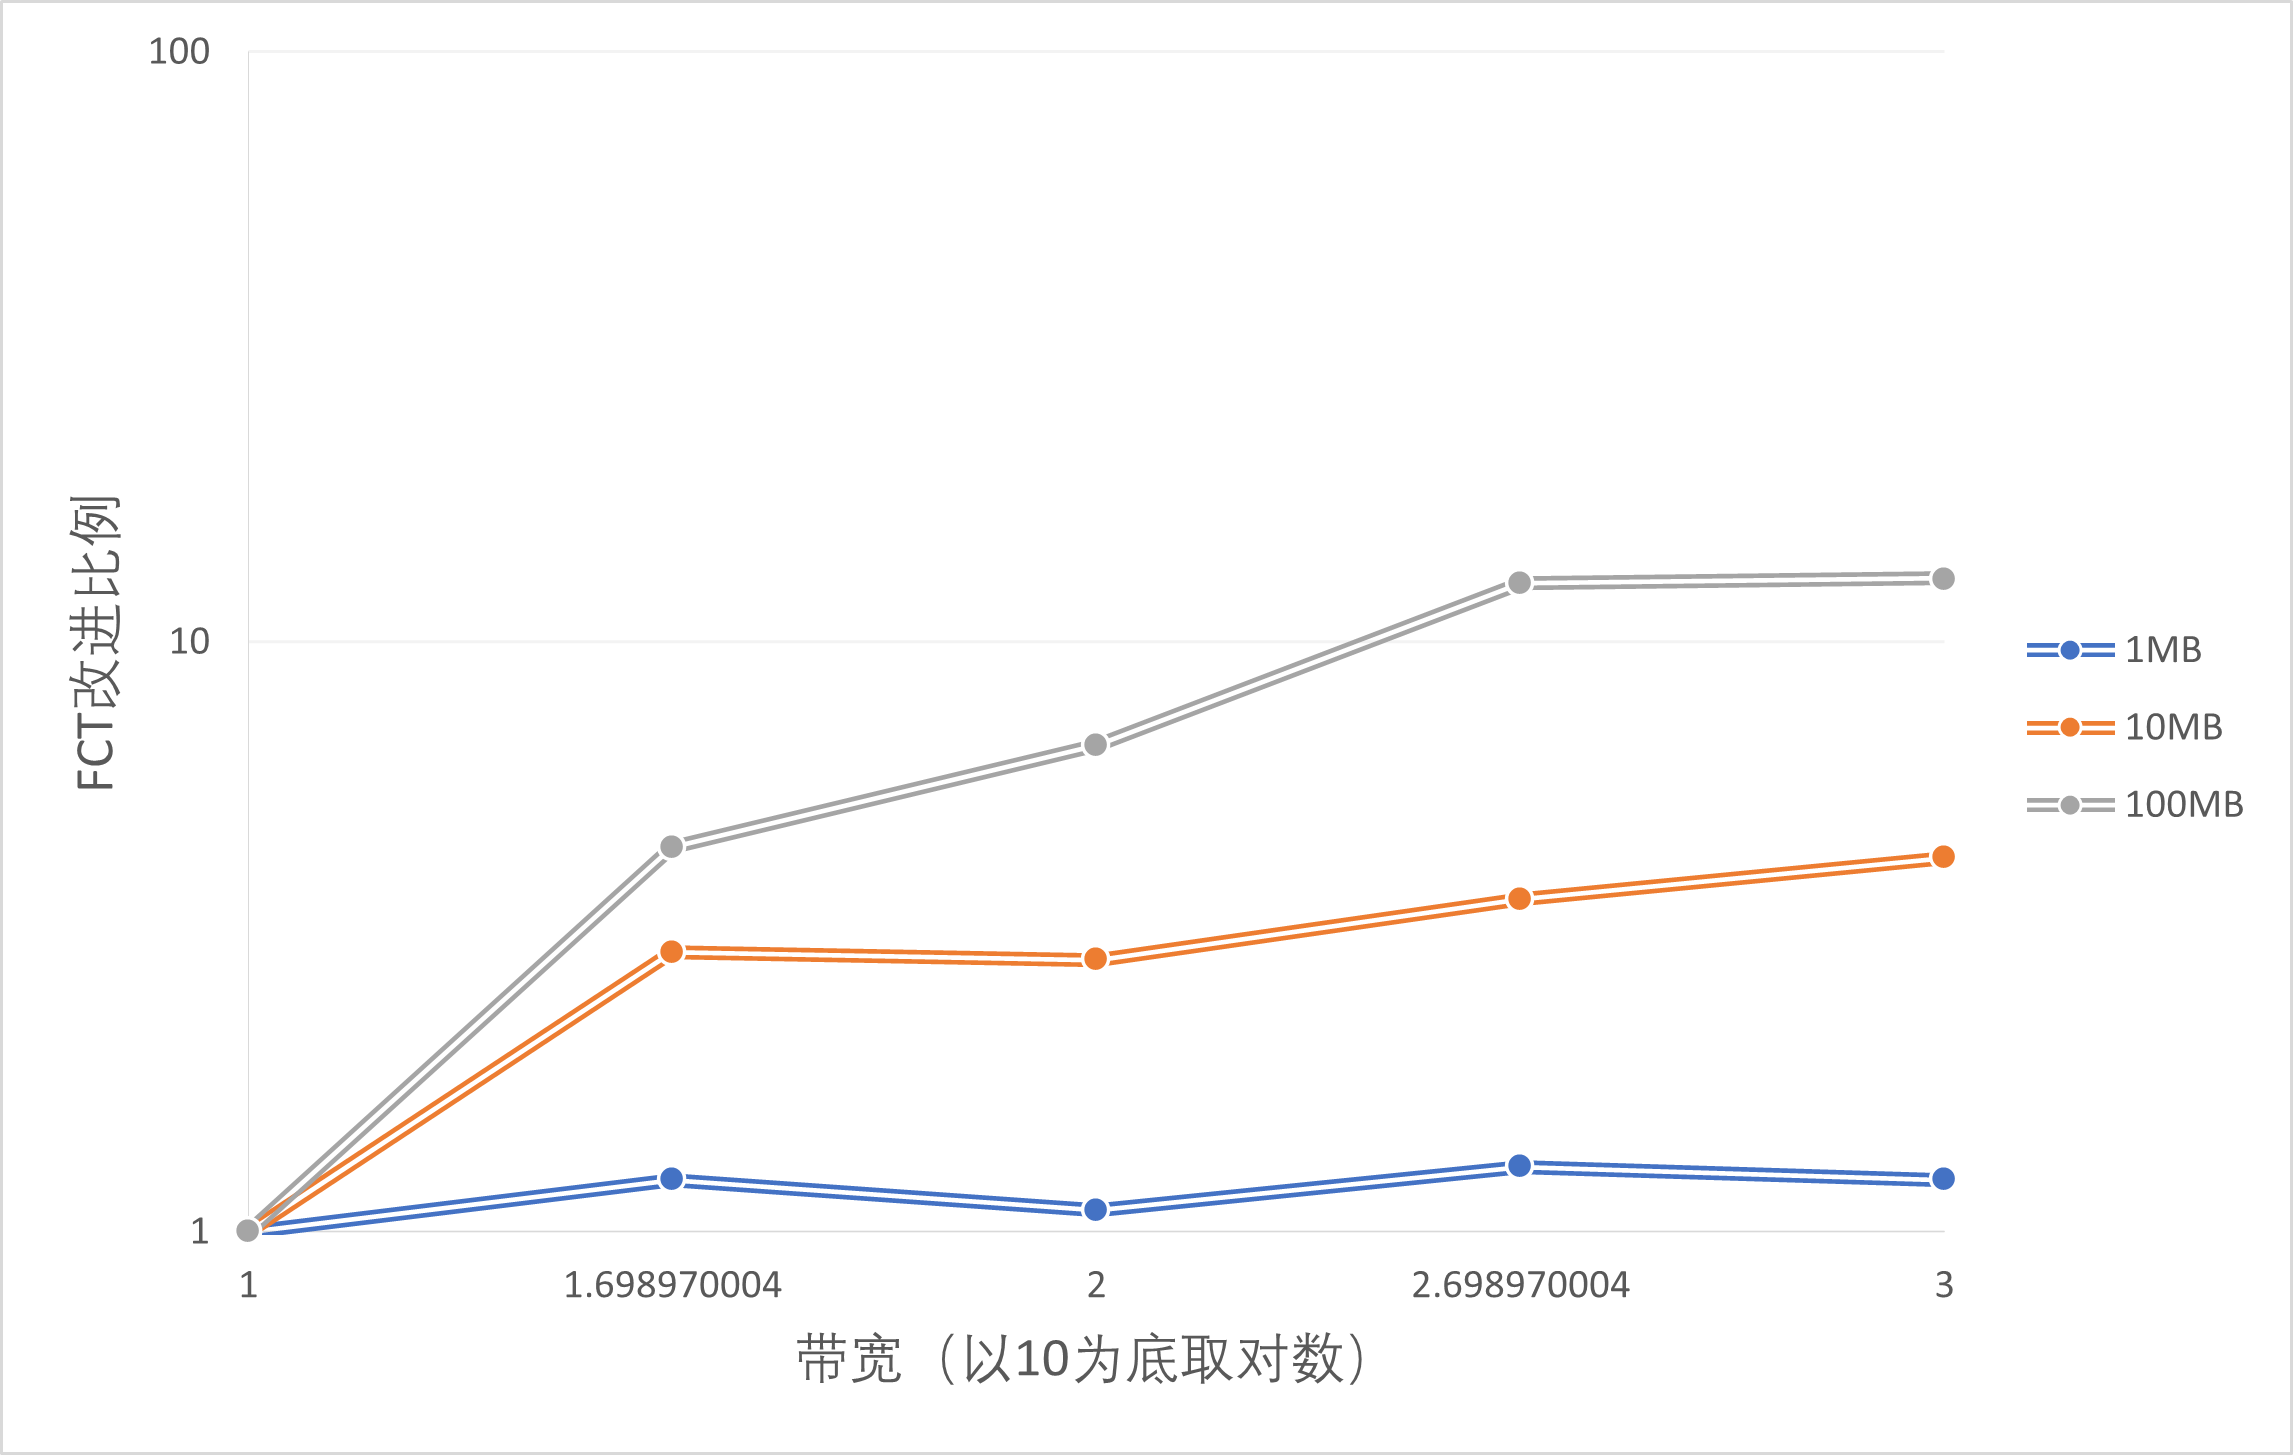
\includegraphics[width=0.8\textwidth]{result2.png}
  \caption{流完成时间实验结果}
\end{figure}

\subsection{实验分析}

这个实验的结果与PPT给出的结果基本一致,只是可能由于网络环境的不同,实验结果有一定的波动。

\begin{enumerate}
  \item 带宽对流完成时间的影响:相同文件大小下,带宽越大,流完成时间大致越短,但是带宽增大对流完成时间的改进比例逐渐减小。
  \item 文件大小对流完成时间的影响:相同带宽之下,文件大小越大,流完成时间越长,这是非常容易理解的,因为文件越大,传输时间越长。此外,文件大小增大可以提高流完成时间的改进比例。
  \item 在下载文件的过程中,有非常明显的下载速率增大的过程,这一过程的时间占比与延迟有关,延迟越大,这一过程的时间占比越大。
  \item 带宽确实是下载速率的理论极大值,但是在实际下载过程中,下载速率并不会达到带宽的极大值,由数据也可以看出。
\end{enumerate}

\subsection{实验解释}

TCP(Transmission Control Protocol,传输控制协议)是一种面向连接的、可靠的、基于字节流的传输层通信协议。在Internet协议族中,TCP层位于IP层之上,负责在数据从源计算机到目标计算机的传输过程中提供可靠的、有序的和无差错的数据传输。TCP的主要特点包括:
\begin{enumerate}
  \item 面向连接:在数据传输之前,发送方和接收方必须建立连接。这个过程通常被称为“三次握手”。这一点之前也提到过。
  \item 可靠传输:TCP使用确认机制来保证数据的可靠传输,即每发送一段数据后,都需要等待接收方的确认。如果发送方在一定时间内没有收到确认,它会重新发送数据。
  \item 流量控制:TCP使用滑动窗口机制进行流量控制,以防止发送方发送数据的速度超过接收方接收数据的速度。
  \item 拥塞控制:当网络拥塞时,TCP会减少数据的发送速度,以减轻网络拥塞。
  \item 数据有序:TCP会对数据进行编号,确保所有数据都能按照发送顺序正确地到达接收方。
\end{enumerate}

TCP的慢启动(Slow Start)是一种拥塞控制策略,用于控制数据包的发送速度,防止网络拥塞。慢启动并不是指启动速度慢,而是指刚开始发送数据时,先发送少量的数据,然后逐渐增加发送速度。当TCP连接刚建立时,发送方的拥塞窗口(cwnd)大小被设置为一个较小的值,通常是MSS(最大段大小)。每当发送方收到一个ACK(确认),它就将cwnd的大小增加1个MSS。这样,cwnd的大小就会在每个RTT(往返时间)内翻倍。当cwnd的大小达到一个阈值(ssthresh,慢启动阈值)时,TCP就会进入拥塞避免阶段,此时cwnd的增长速度会减慢。如果发生了超时或者丢包,TCP就会将ssthresh设置为当前cwnd的一半,并将cwnd重新设置为1个MSS,然后重新进入慢启动阶段。通过这种方式,TCP可以在保证网络稳定的同时,尽可能快地发送数据。

\section{实验总结}

本次实验主要是通过wireshark抓包工具,观察ARP、DNS、TCP和HTTP协议的工作过程,以及通过fct_exp.py脚本,查看流完成时间,分析带宽、延迟和文件大小对流完成时间的影响。通过这两个实验,我对网络协议的工作原理和流完成时间的影响因素有了更深入的了解。这些知识都是我之前从未了解过的,通过实验,我期望能够继续加深学习计算机网络的知识,提高自己的实践能力。
\end{document}